\section{Documentation of the current performance}

To properly measure the performance of our program, we needed to document the execution time of the program.
We created a timer class and implemented it into the program to measure it's performance. 

\begin{figure}[h]
    \caption{Timer.java}
    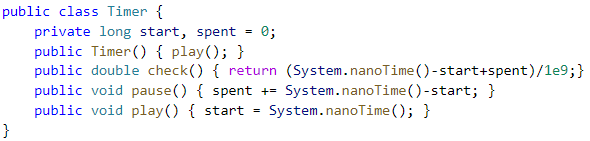
\includegraphics[]{figures/Figure-1.png}
    \label{fig:timer-class}
\end{figure}

\begin{figure}[h]
    \caption{Main.java}
    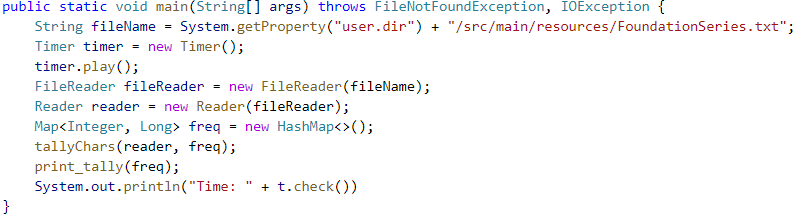
\includegraphics[]{figures/Figure-2.png}
    \label{fig:main-cass}
\end{figure}

With our timer implemented, we then ran the program for a total of 10 times and took the average of our timings to present a baseline of performance.\\\\

\begin{lstlisting}[]
Run 1:  152.073 ms
Run 2:  104.019 ms
Run 3:  66.9943 ms
Run 4:  88.3265 ms
Run 5:  64.8921 ms
Run 6:  52.9183 ms
Run 7:  53.6571 ms
Run 8:  53.3412 ms
Run 9:  96.7388 ms
Run 10: 87.2514 ms
\end{lstlisting}

\pagebreak
As we can see by our timings, the time to execute the program varies greatly.\\
The reason our timings are different for each run, is due to the pc running other processes during the test. In hindsight we should have run the test in a virtual environment to prevent any outside interferences, however by running the code 10 times and getting the average runtime we circumvent some of these interferences to get a clearer result.\\

We can now use our data to do a couple of different calculations to get an even even clearer picture of our programs performance before we improve upon it.\\
\begin{lstlisting}[]
Count:                  10
Sum:                    820.2117
Mean:                   82.02117
Variance:               866.8134585601
Standard Deviation:     29.441695918546
\end{lstlisting}